
les besoins des architectures (from IoT to the cloud)-> présenter différents aspects genre object to object / object to gateway / object to cloud et réciproquement

\begin{resume}
	Dans l'ensemble des éléments qui composent les systèmes informatiques, les réseaux informatiques sont parmi les éléments qui sont les plus exposés et impactés par l'hétérogénéité. Cette hétérogénéité peut se présenter sous différéntes formes : diversité d'équipements et de technologies, variations de performance et disponibilité (volatilité), limitations liées aux caractéristiques physiques ou à la capacité des ressources, etc. 
	
	Si cette hétérogénéité doit être prise en compte lors du développement de systèmes et applications, il s'avère souvent que les solutions se limitent à pallier les éventuels problèmes. Les travaux que j'ai mené dans le domaine de l'hétérogénéité des réseaux visent la compréhension des facteurs liés à l'hétérogénéité, leur caractérisation et aussi l'optimisation de l'usage des ressources afin de rendre les systèmes et applications plus performants et fiables.
	
	L'une des premières étapes dans l'étude de l'hétérogénéité requiert l'observation et l'analyse des communications réseau afin de modéliser leur fonctionnement et ainsi permettre une estimation de leurs performances. Cette étude cache néanmoins une grande complexité car même sur un petit ensemble de ressources la variation de certains facteurs peut créer un nombre important de situations, chacune avec un modèle de communication différent. Afin de permettre l'application pratique de cette modélisation de performance nous devons non seulement être en mesure de découvrir la topologie du réseau, mais aussi de pouvoir quantifier les différents facteurs et émettre des hypothèses sur les modèles de communication observés. 
	
	Un mécanisme très utile dans la réduction de la complexité de la modélisation des communications réside dans la classification et catégorisation des ressources observées. Non seulement cela permet de se concentrer sur des modèles "type" qui représentent convenablement des ensembles de ressources, comme aussi on ouvre la possibilité d'utiliser ces informations dans le but d'optimiser les échanges entre les applications.
	
	Dans certains cas, cependant, juste la connaissance des profils de performance peut s'avérer insuffisante, notamment lorsque les applications ont des besoins de fiabilité accrus. Ainsi, l'hétérogénéité dans les réseaux doit aussi s'intéresser à l'observation des ressources afin de détecter des éventuelles défaillances, et de les signaler aux applications et systèmes, qui pourront ainsi réagir et prendre des mesures nécessaires pour assurer ses engagements de fiabilité. 
	
	Dans cette première partie, la Section \ref{sec:reseaux-model} présente les travaux qui ont été menés sur la modélisation et l'évaluation des performances de communication des réseaux. La Section \ref{sec:reseaux-topo} présente les travaux sur la découverte de la topologie et la subséquente classification des ressources. Finalement, la Section \ref{sec:reseaux-defaillances} présente les travaux sur la détection de défaillances. Tous ces éléments sont connectés aux travaux qui seront présentés dans les chapitres suivants.  
	%Cette première partie regroupe les travaux que j'ai menés sur la
	%structuration des systèmes distribués à l'aide de marches
	%aléatoires. Ils constituent la continuité de ceux menés durant ma
	%thèse.
	%
	%J'exploite les marches aléatoires selon deux axes. Le premier consiste
	%à n'utiliser que la circulation, sans collecte d'informations au cours
	%du déplacement. Le second consiste à combiner les concepts de marche
	%aléatoire et de mot circulant, afin d'exploiter l'historique des
	%déplacements du jeton.
	%
	%La première approche m'a permis de définir un algorithme rapide de
	%construction et de maintenance d'un arbre couvrant sur un système
	%distribué. Cette construction est auto-stabili\-sante, et garantit
	%donc la tolérance aux fautes transitoires qui peuvent affecter le
	%système.
	%
	%Dans la seconde approche, l'historique des déplacements est conservé
	%dans le jeton, mais n'a aucun impact sur la circulation qui reste
	%aléatoire sans mémoire. Le contenu du jeton est analysé et exploité,
	%afin de permettre la construction d'arbres couvrants sur chaque
	%site. Je propose différents algorithmes auto-stabilisants de gestion
	%et de correction du contenu du jeton et de sa circulation. Je dérive
	%de cette circulation un algorithme auto-stabilisant garantissant la
	%$k-$exclusion mutuelle.
	%
	%La majorité des travaux présentés dans cette partie, ont été réalisés
	%en collaboration avec Alain Bui, professeur à l'université de Reims
	%Champagne-Ardenne, et Thibault Bernard, dont je co-encadre une partie
	%des travaux de thèse avec Alain Bui.
	
\end{resume}

\section{Introduction} \label{sec:intro}

Avec l'augmentation exponentielle du nombre de dispositifs informatiques de proximité (smartphones, tablettes, nano-ordinateurs, etc.), il est important de comprendre comment organiser ces ressources et comment gérer l'information de manière adaptée à ces environnements pervasifs. 
%En effet, notre vie quotidienne présente de plus en plus d'appareils connectés pour suivre notre santé et nos mouvements, la sécurité de nos maisons ou le niveau d'humidité du sol pour nos plantes. 
%À nos jours, les principales limitations % d'utilisation de ces dispositifs ne sont pas liées à leur capacité de communication (WiFi, Bluetooth, etc.), mais surtout à la difficulté d'une application exploiter l'interconnexion à d'autres appareils or cette frontière est en train de tomber avec l'avènement de l'internet des Objets (\textit{Internet of Things} - IoT). 
Cette augmentation est liée, entre autres, à l'avènement de l'Internet des Objets (\textit{Internet of Things} - IoT). L'IoT représente une nouvelle tendance de l'industrie informatique où l'environnement physique est peuplé d'objets interconnectés et communicants qui interagissent les uns avec les autres et avec l'environnement lui-même. La force de ce concept réside dans l'intégration transparente des capteurs, des actionneurs et d'autres dispositifs, ce qui permet l'interaction et la collecte d'informations à grande échelle.

Plusieurs facteurs ont contribué au développement de l'Internet des Objets, dont l'augmentation de la bande passante et de la puissance de calcul des appareils, couplés avec un coût décroissant de capteurs \cite{Jones2014}. De nos jours, il est possible d'équiper la quasi-totalité des dispositifs quotidiens d'une interface sans fil, rendant ainsi possible l'interaction entre eux \cite{Paridel2010}. De telles capacités de communication ouvrent d'innombrables possibilités dans plusieurs domaines tels que la santé et les villes intelligentes, mais soulève également plusieurs défis concernant l'évolutivité, l'hétérogénéité et la dynamicité du réseau. Les principales limitations d'utilisation de ces dispositifs à nos jours ne sont pas liées à leur capacité de communication (WiFi, Bluetooth, etc.), mais surtout à la difficulté d'une application à mieux tirer profit de cette interconnexion à d'autres appareils. Le  potentiel de l'IoT ne sera pleinement atteint que si les données issues de l'IoT puissent être analysées et explorées convenablement par les applications.

Actuellement, l'agrégation et l'analyse des données IoT sont effectuées principalement sur les infrastructures déportées de type \textit{cloud computing}. Plusieurs travaux \cite{Miorandi2012, Gubbi2013, Fazio2015} comptent sur ces infrastructures car elles offrent de la puissance de calcul  et de la flexibilité pour l'exécution de services et applications \cite{Serrano2013}. Malgré ses avantages, les plates-formes de type \textit{cloud} ont aussi quelques inconvénients importants. En effet, le transfert de données %provenant d'environnements IoT au cloud 
peut être considérablement coûteux et prendre du temps. En outre, les applications qui dépendent entièrement des services distants peuvent échouer si la connexion est défectueuse ou trop lente.

Par conséquent, nous devons repenser la façon de transmettre, de stocker et d'analyser les données dans ces environnements. Les architectures réseau traditionnelles ne sont pas préparées pour l'hétérogénéité qui caractérise l'IoT (à la fois sur les capacités de calcul, de mémoire, d'autonomie et de communication), ni sont elles préparées pour la nature spontanée de leurs interactions. Cette préoccupation a conduit les chercheurs à développer une série de solutions alternatives au \textit{cloud computing}, telles que les grilles pervasives \cite{Parashar2010}, le \textit{mobile edge computing} \cite {Dey2013,MEC,Satyanarayanan09}, le \textit{fog computing} \cite{Bonomi2012} ou bien le \textit{edge-centered computing} \cite{Lopez2015}. Toutes ces alternatives partagent un même objectif : utiliser la puissance de calcul des dispositifs environnants pour effectuer des tâches habituellement déléguées à une installation distante. 

Pour répondre aux défis de l'IoT, ce travail préconise le développement de plates-formes multi-échelle capables d'assurer la coordination et la redistribution des tâches entre les appareils (en fonction de leurs capacités), améliorant ainsi l'utilisation des ressources et la qualité de service. Nous présentons des solutions architecturales et pratiques à mettre en \oe{}uvre pour la création d'une plate-forme multi-échelle adaptée à l'IoT, en utilisant comme base une plateforme de dispositifs reliés par un réseau P2P.

La suite de cet article est organisée comme suit : la Section \ref{sec:definitions} présente l'état de l'art sur le calcul dans les environnements pervasifs, ainsi que la définition de l'informatique multi-échelle. La Section \ref{sec:requeriments} analyse les principales exigences pour un cadre multi-échelle et illustre comment une telle approche est mise en \oe{}uvre sur la plate-forme de calcul CloudFIT. Finalement, la Section \ref{sec:concl} présente nos conclusions et travaux futurs.


\section{État de l'Art}\label{sec:definitions}

La diffusion des dispositifs de proximité avec des capacités de calcul non-négligeables (smartphones, tablettes, ordinateurs portables et nano-ordinateurs tels que le Raspberry Pi) encourage l'intégration de ces dispositifs dans le traitement des données. %Par conséquent, des travaux tels que les grilles pervasives \cite{Parashar2010}, le \textit{mobile edge computing} \cite {Dey2013,MEC,Satyanarayanan09}, le \textit{edge-centered computing} \cite{Lopez2015} ou bien le \textit{fog computing} \cite{Bonomi2012} ont essayé de placer les applications et les services plus près de l'utilisateur final.


Les travaux sur l'\textit{edge computing} et le \textit{fog computing} partagent souvent les mêmes définitions \cite{Vermesan}. En effet, le \textit{fog computing} a été défini par CISCO \cite{FogCISCO} comme "un paradigme qui étend le \textit{cloud computing} et des services à la périphérie du réseau", tandis que le \textit{(mobile) edge computing} vise à transformer les stations de base proches en "centres de services intelligents capables de fournir des services hautement personnalisés" \cite{Vermesan}. Des exemples de \textit{edge/fog} comprennent des services \textit{fog} \cite{Bonomi2012} et les \textit{cloudlets} \cite{Satyanarayanan09}, tous les deux proposant le déploiement des serveurs de proximité offrant des services avec une latence réduite. A quelques exceptions près, comme \cite{Dey2013}, ces travaux considèrent que les dispositifs IoT ne contribuent pas à l'effort de calcul, restant dépendants d'un service tiers (à proximité ou à distance).

Garcia Lopez et al. \cite{Lopez2015} explorent une autre facette de l'\textit{edge computing} en se concentrant sur le rôle de l'homme dans la boucle de contrôle. En effet, ces auteurs affirment la nécessité de recentrer le contrôle sur les équipements situés au bord du réseau, au lieu de simplement les considérer comme une première couche de calcul reliée à un réseau plus grand et plus puissant. %Ces auteurs donnent une attention particulière à l'interaction humaine, qui revient au centre des décisions. 
Malheureusement, dans cette définition les dispositifs IoT ne contribuent pas non plus aux efforts de calcul, étant considérés comme des capteurs/actionneurs pilotés par les interactions entre l'homme et l'\textit{edge}.

Bien que ces travaux préconisent la nécessité d'un environnement informatique de proximité, ils oublient souvent de détailler l'interconnexion ou les exigences de coordination entre les processus. Cela est particulièrement nécessaire dans l'optique de l'IoT, qui impose des défis importants pour l'évolutivité, la dynamicité et l'hétérogénéité des ressources. Afin de gérer efficacement les environnements pervasifs IoT, nous proposons l'utilisation de stratégies multi-échelles pour la gestion et la coordination des périphériques.

Dans la littérature nous trouvons, par exemple, la notion de grille pervasive \cite{Parashar2010}, qui vise l'intégration des dispositifs de détection/d'actionnement ainsi que des systèmes de haute performance classiques. Ces grilles reposent sur l'utilisation des ressources habituellement sous-utilisés, composant ainsi une plate-forme de calcul dynamique \cite{Steffenel2015Roma}. En effet, les grilles pervasives offrent la possibilité d'intégrer les différents ressources disponibles allant des petits appareils de type Raspberry Pi jusqu'aux machines virtuelles déployées sur les infrastructures d'un datacenter. Pour l'IoT, les grilles pervasives représentent une opportunité de déployer des tâches informatiques sur des ressources situées à proximité des dispositifs IoT, minimisant ainsi le transfert de données vers un réseau distant. De plus, selon les besoins, ces tâches peuvent être allouées aux ressources avec la capacité de calcul adéquate à chaque service, sans avoir à externaliser les données et les services.

Un autre avantage des grilles pervasives est son indépendance par rapport à des architectures et services opérateur. Malgré l'appel à la décentralisation et à l'affranchissement du "tout cloud" prôné par les pemiers travaux sur l'edge-computing et le fog-computing, nous observons une "appropriation" de ces concepts par les grands opérateurs du marché télécom et cloud tels que Cisco, Intel ou Microsoft, réunis par exemple au sein de l'Open Fog Consortium\footnote{\url{http://www.openfogconsortium.org/}} afin de créer une architecture de référence pour le fog computing. Bien que de telles initiatives sont nécessaires pour la maturation d'une technologie, elles sont souvent source de contraintes au déploiement de plates-formes légères, ce qui est notre objectif principal.

Afin de répondre aux différents besoins des architectures et applications IoT, les grilles pervasives doivent être enrichies avec le concept des systèmes multi-échelle. Les \textit {systèmes multi-échelles} sont des systèmes distribués où les services sont organisés en couches à travers une ou plusieurs dimensions (dispositifs, réseau, localisation géographique, etc.), chaque couche fournissant un niveau de service supplémentaire qui peut être consulté en fonction du contexte de l'appareil \cite{Rottenberg2012,Rottenberg2014}.  En vertu de cette approche, des actions primaires peuvent être décidées/interprétées à proximité, tandis qu'une analyse plus poussée de l'information peut être effectuée par des serveurs externes. Cette analyse stratifiée peut également être utilisée pour renforcer les aspects liés à la vie privée comme, par exemple, l'anonymisation des données qui seront externalisés. Nous croyons que ce concept offre plusieurs niveaux de granularité et d'interconnexion nécessaires à l'autonomie des dispositifs IoT et permet des services plus réactifs et de meilleure qualité. Ceci est notamment utile dans des domaines tels que la domotique, où l'adaptation au contexte et le respect de la vie privée sont de facteurs clé.

Dans la section suivante nous énumérons certaines exigences pour le développement d'une plate-forme informatique multi-échelle.

\section{Calcul Multi-Échelle}\label{sec:requeriments}

Comme indiqué dans la section précédente, la plupart des travaux sur le \textit{edge/fog computing} ont la tendance à faire une distinction entre l'utilisateur final (ou les périphériques finaux) et les dispositifs qui se trouvent sur la frontière la plus proche de l'Internet/\textit{cloud}. Dans de telles approches, les appareils IoT sont des simples clients des services déployés dans un voisinage proche. Contrairement au \textit{fog/edge computing}, les grilles pervasives supposent que tous les dispositifs peuvent contribuer au calcul des tâches selon leurs propres capacités et ressources disponibles. Les dispositifs IoT peuvent alors devenir des acteurs actifs de l'environnement et non seulement des clients passifs. Les concepts de grilles pervasives et de calcul multi-échelle peuvent ainsi être utilisés pour intégrer les dispositifs IoT dans l'environnement informatique.
%, et par conséquent cette section décrit un ensemble d'exigences pour permettre cette intégration.

Cependant, afin que les applications puissent profiter pleinement de ces environnements, différents challenges doivent être relevés. 
Dans ce travail, nous analysons un ensemble d'exigences qui nous paraissent essentielles pour cette intégration et nous illustrons leur prise en charge par une %Dans ce travail nous présentons également des directions pour la mise en place d'une 
plate-forme de calcul multi-échelle basée sur CloudFIT \cite{Steffenel2015Roma}. CloudFIT est un middleware de calcul P2P basé sur le paradigme FIIT (\textit{Finite Independent Irregular Tasks}). La version actuelle prend en charge le système %FreePastry \footnote{\url{http://www.freepastry.org/}} et 
TomP2P \footnote{\url{http://tomp2p.net}} ainsi que son API DHT (basée sur Kademlia), offrant des possibilités intéressantes pour la gestion des données. CloudFIT est développé en Java et peut donc être déployé sur une large gamme de dispositifs (une version Android est en cours de développement). Afin de rendre son déploiement simple et rapide, nous avons pris soin de minimiser les dépendances envers les bibliothèques tiers, ce qui permet le lancement de la plate-forme avec un simple fichier \textit{jar}.

La flexibilité de lancement de CloudFIT permet son exécution directement sur certains appareils IoT récents, souvent localisés au bord du Edge. Dans le cas des capteurs isolés ou de micro-contrôleurs de type Arduino, incapables de tourner le code Java, CloudFIT peut servir de \textit{gateway}, grâce à une interface front-end permettant le stockage des données et le déclenchement d'actions, comme illustré sur le côté gauche de la Fig. \ref{fig:CloudFit}.


\begin{figure}
	\begin{center}
		%\vspace{-0.3cm}
		\includegraphics[width=1\linewidth]{img/CloudFITstack-IoT}
		%\vspace{-0.4cm}
		\caption{La pile d'exécution CloudFIT et l'interface pour les dispositifs IoT}\label{fig:CloudFit}
		%\vspace{-0.7cm}
	\end{center}
\end{figure}


Les prochaines sections décrivent ainsi les défis pour la mise en place d'une plate-forme multi-échelle et comment nous avons adapté CloudFIT à ces fins.

\subsection{Communication, coordination et clustering}

L'un des principaux défis avec le calcul multi-échelle dans un environnement IoT est celui de permettre à la fois un contrôle précis sur les ressources et une interaction simplifiée avec le reste du réseau. En effet, les environnements IoT se caractérisent par leur échelle très variable, pouvant varier de quelques objets à plusieurs milliards. En concevant chaque couche comme un cluster, nous pouvons utiliser un réseau P2P soutenant le déploiement de chaque couche. Cependant, les réseaux P2P les plus connus organisent les n\oe{}uds indistinctement de leur emplacement réel, ce qui empêche l'établissement d'un regroupement de n\oe{}uds pour fournir des services à faible latence. Pour contourner ces inconvénients, nous considérons que le réseau P2P doit être enrichi par l'utilisation de techniques de \textit{clustering}. En effet, le regroupement des ressources sous la forme de \textit{clusters} est une manière efficace pour organiser les couches de calcul multi-échelle et ainsi fournir une base de coordination pour le déploiement efficace des services.

Plusieurs approches de clustering sont proposées dans la littérature \cite{Johnen2011} et utilisées, par exemple, pour  le routage des informations dans les réseaux de capteur sans fil. La plupart des algorithmes de clustering utilisent des paramètres simples comme la densité du réseau environnant, choisissant un \textit{cluster-head} en fonction de leurs identités uniques (ID). Malheureusement, ces métriques sont insuffisantes pour assurer le clustering dans un scénario hétérogène comme celui de l'IoT, vu qu'elles ne permettent pas d'exprimer les besoins du calcul multi-échelle. Au contraire, le regroupement des n\oe{}uds doit être défini à la fois de manière à co-localiser les données et les ressources de calcul nécessaires et aussi à définir des couches de calcul reliant les dispositifs proches et plus éloignés (jusqu'au cloud). Ainsi, afin de s'adapter à l'hétérogénéité des environnements pervasifs et l'IoT, les métriques de clustering doivent être étendues pour inclure des informations de contexte telles que la proximité, les capacités informatiques et de stockage des appareils, la fiabilité et même la niveau d'autorisation/confiance des n\oe{}uds collaborateurs.
 
 
 \begin{figure}[!ht]
 	%\renewcommand{\figurename}{Figura}
 	\centering
 	%\vspace{-0.3cm}
 	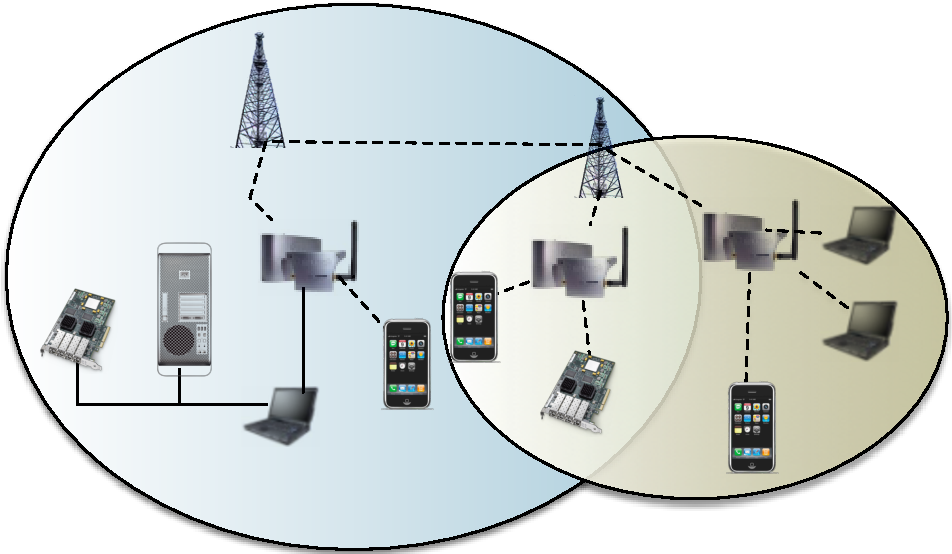
\includegraphics[width=1\linewidth]{img/antennes2.pdf}
 	%\vspace{-0.2cm}
 	\caption{Des communautés interconnectées dans une plate-forme multi-échelle}
 	\label{fig:antennes}
 	%\vspace{-0.5cm}
 \end{figure}

Dans le cas de CloudFIT, ce clustering peut être mis en \oe{}uvre grâce au concept de \textit{communautés}, des sous-ensembles de n\oe{}uds qui peuvent être adressés séparemment et donc utilisés pour répartir/cloisonner les opérations. Dans le cas d'un clustering automatique, la liste de membres est gérée par le \textit{cluster-head}. Les membres de la liste peuvent donc être contactés en utilisant des procédures spécifiques telles que les diffusions structurées de TomP2P. Bien entendu, un n\oe{}ud peut appartenir à plusieurs communautés, permettant à des données et des tâches de circuler entre les différentes couches multi-échelle, comme illustrée en Fig. \ref{fig:antennes}. 
Cette organisation à plusieurs niveaux en fonction du contexte des ressources disponibles permettrait de mieux coordonner la communication entre ces ressources et d'ainsi mieux gérer la variabilité d'échelle de ces environnements. 



\subsection{Contexte et ordonnancement}

Dans les environnements pervasifs, la sensibilité au contexte est essentielle pour la planification des tâches vu que la performance varie beaucoup d'un appareil à l'autre \cite{Dey2013}. Les informations contextuelles telles que la puissance de calcul, la mémoire disponible et l'espace de stockage peuvent être utiles pour améliorer l'exécution en assignant des tâches aux dispositifs les plus adéquats. Avec d'autres paramètres tels que la proximité géographique, la latence réseau et le niveau de fiabilité d'un n\oe{}ud, la sensibilité au contexte est un outil nécessaire à la clusterisation des n\oe{}uds et à la composition de services multi-échelle.

Bien que la collecte d'informations de contexte et sa mise en \oe{}uvre est au-delà de la portée de cet article, il faut noter que les algorithmes d'ordonnancement doivent néanmoins être assez permissives, avec l'exclusion des n\oe{}uds uniquement lorsque les exigences spécifiques de l'application ne sont pas respectées (par exemple, un minimum de capacité mémoire). 
%En effet, nous ne savons pas quels appareils peuvent être présents dans le réseau et, par conséquent, 
En effet, la dynamicité des environnements pervasifs due entre autres à la mobilité de certains appareils, rend particulièrement difficile d'anticiper quelles ressources seront disponibles et dans quelle mesure elles le seront. Dans ces conditions,  
il est préférable d'avoir des n\oe{}uds lents mais qui contribuent à l'effort que d'avoir un blocage par manque de ressources ou une surcharge trop importante des n\oe{}uds rapides \cite{Cassales2016,Wang2015}.   


\begin{figure} [!hbt]
	\centering
	%\vspace{-0.3cm}
	\includegraphics[width=1\linewidth]{img/CollectorUML2.pdf}
	%\vspace{-0.2cm}
	\caption{Architecture pour un collecteur de contexte \cite{Cassales2015202}}
	\label{fig:CollectorDiag}
	%\vspace{-0.5cm}
\end{figure}


Les applications CloudFIT étant décrites par un ensemble fini de tâches qui peuvent être réparties entre les n\oe{}uds, des informations de base telles que le nombre de tâches parallèles qu'un n\oe{}ud peut supporter sont déjà utilisées par l'ordonnanceur. Si l'ordonnanceur par défaut utilise une approche totalement distribuée (exécution \textit{best-effort} associée à la diffusion des tâches finies), il peut être enrichi avec d'autres éléments tels que la mémoire disponible ou la vitesse relative des CPUs. La collecte de ces éléments peut se faire grâce au collecteur de contexte que nous avons proposé et utilisé dans \cite{Cassales2016}, présenté sur la figure \ref{fig:CollectorDiag}.



\subsection{Accès aux données}
%
Dans le cadre du traitement de données issus des dispositifs de l'IoT, un autre facteur à prendre en compte est celui de la performance liée à l'accès et à la gestion des données. En effet, la plupart des opérations impliquent la collecte, la transformation et l'analyse des données, et les plates-formes telles que Apache Hadoop se sont illustrées par leur capacité d'optimiser l'accès aux données en plaçant les tâches préférentiellement là où les données sont présentes (grâce au concept de la \textit{data locality}). 

Dans le passé \cite{Steffenel2015Roma} nous avons déjà mené des expérimentations avec CloudFIT démontrant que des performances similaires ou supérieures à celles de Apache Hadoop pourraient être atteintes avec un système P2P, comme illustré en Fig. \ref{fig:Hadoop}. Bien que ces résultats ont été positifs, nous avons observé deux points qui pourraient être encore améliorés : la surcharge de gestion des données sur un noeud et la prise en charge de la \textit{data locality}. 

\begin{figure}[!ht]
	%\renewcommand{\figurename}{Figura}
	\centering
	%\vspace{-0.3cm}
	\includegraphics[width=1\linewidth]{img/CloudFIT-mesures.pdf}
	%\vspace{-0.2cm}
	\caption{Comparaison des temps d'exécution de WordCount avec CloudFIT et Hadoop}
	\label{fig:Hadoop}
	%\vspace{-0.2cm}
\end{figure}


Dans le premier cas, nous avons constaté un fort écart de performances d'accès aux données lorsque nous déployons CloudFIT  dans un environnement hétérogène. Ces écarts de performance sont en effet une combinaison de la vitesse d'accès aux données et de la surcharge de gestion des systèmes de stockage (voir aussi les limitations physiques de stockage), et affectent notamment les dispositifs de faible capacité situés à la frontière de l'Edge Computing. Ainsi, par exemple, un Raspberry Pi est fortement penalisé par la vitesse et la capacité de stockage de sa carte SD, malgré une capacité de calcul suffisante (notamment en utilisant tous ses coeurs de calcul).  Afin de contourner cette limitation, nous avons modifié la couche de stockage afin que les n\oe{}uds puissent choisir d'agir seulement en tant que clients distants. Ces n\oe{}uds peuvent donc interroger la surcourche de stockage P2P via le réseau mais ils ne sont plus obligés à gérer le stockage, réduisant leur surcharge et aussi leur utilisation du disque.

Por ce qui est de la prise en charge de la \textit{data-locality}, c'est un problème plus général qui affecte la plupart des architectures de stockage P2P. En effet, les API de stockage P2P sont souvent basés sur les tables de hachage distribuées (DHT). Ces DHTs sont conçues de manière à répartir les données sur le réseau et les répliquer lorsque cela est possible, notamment afin d'éviter la perte de données en cas de désabonnement (\textit{churn}). Un inconvénient de cette procédure est qu'on observe une perte d'information concernant la localisation des données \cite{Wu2005}, rendant difficile l'optimisation des transferts réseau. 

A l'instar d'autres systèmes de P2P, La bibliothèque Tom P2P utilisée par CloudFIT ne permet pas encore à un n\oe{}ud de faire la différence entre les données locaux ou distants. Nous sommes en contact avec l'équipe de développement TomP2P afin d'intégrer une telle fonctionnalité dans les futures versions, mais en attendant nous avons développé une stratégie pour renforcer la proximité des données grâce à un calcul personnalisé de la clé de localisation des ressources. 

Ceci est possible car contrairement à la plupart des systèmes de P2P qui ont seulement une clé de hachage unique, TomP2P identifie les ressources par quatre clés différentes $\{k_l,k_d,k_c,k_v\}$, selon l'hiérarchie suivante : 
\begin{itemize}
	\item \textit{$k_l$} - clé de localisation, utilisée pour la localisation d'une ressource dans la DHT
	\item \textit{$k_d$} - clé de domaine, fonctionne comme une clé d'authentification, permet la séparation des données
	\item \textit{$k_c$} - clé de contenu, permet d'identifier une ressource. Par défaut est identique à la clé de localisation 
	\item \textit{$k_v$} - clé de version, permet la gestion de versions multiples d'une ressource
\end{itemize} 

La clé de localisation est celle qui s'approche le plus des clés DHT traditionnelles, ayant par fonction l'association d'une ressource (copie primaire ou index) au n\oe{}ud avec l'ID le plus proche. Sans aucune instruction supplémentaire, la clé de localisation et la clé de contenu sont les mêmes, mais peuvent être différentes par exemple en cas de collision (deux ressources avec la même clé de localisation).

La clé de domaine est liée à un mécanisme d'authentification simple de TomP2P, son but étant de renforcer le cloisonnement des données des différents clients (cette authentification doit être renforcée par l'utilisation de la cryptographie afin de garantir une véritable confidentialité). Dans le cas de CloudFIT, la clé de domaine est utilisée comme un \textit{namespace} pour la séparation des données de différents communautés ou jobs de calcul. 

Finalement, la clé de version permet la coexistence de différentes versions d'une ressource, ce qui permet une meilleure gestion des données "mutables", avec par exemple un accès à l'historique des modifications ou ll'écriture en parallèle d'une ressource par plusieurs n\oe{}uds. Cette clé de version est utilisée dans les nouvelles versions de l'application MapReduce développée sur CloudFIT.

Ainsi, afin de renforcer la \textit{data locality}, nous avons travaillé sur le découplage entre la clé de localisation et la clé de contenu grâce à une double fonction de hachage. Dans un premier moment, la clé de contenu est obtenue avec une méthode de hachage classique. Ensuite, la clé de localisation est calculée en faisant une association limitée aux ID des n\oe{}uds d'une communauté. La Fig. \ref{fig:hash} montre l'exemple de cette cartographie en calculant la clé de localisation d'une ressource $r_3$ par rapport à une communauté $Comm_1$.

\begin{figure}[!ht]
	%\renewcommand{\figurename}{Figura}
	\centering
	%\vspace{-0.3cm}
	\includegraphics[width=1\linewidth]{img/hashing.pdf}
	%\vspace{-0.2cm}
	\caption{Cartographie des ressources renforçant la data-locality}
	\label{fig:Hadoop}
	%\vspace{-0.2cm}
\end{figure}

Cette cartographie augmente la probabilité que la copie primaire d'une donnée se trouve parmi les membres de la communauté, sans pour autant empêcher la réplication des données sur d'autres n\oe{}uds. Cette approche est aussi tolérante aux variations du nombre de membres de la communauté : en cas de disparition d'un n\oe{}ud, c'est une réplique qui prend le relais ; en cas d'un nouveau membre, celui-ci sera intégré à la fonction de hachage normalement.   
